\documentclass{article}
\usepackage{hyperref}
\hypersetup{colorlinks=true,urlcolor=blue}
\usepackage{listings}
\usepackage{geometry}
\geometry{margin=1in}
\usepackage{graphicx}
\graphicspath{ {./hw1/} }
\begin{document}
\title{BMI 203: Algorithms - Homework 1}
\author{Laurel Estes}
\maketitle
\section{Implement BubbleSort and QuickSort}
I implemented BubbleSort with a nested for-loop, as follows:
%\vspace{0.5cm}
\begin{lstlisting}[language=Python]
def bubblesort(x):
    for n in range(len(x)):
    	#now comparing adjacent, so iterate up to 2nd-to-last
        for i in range(len(x)-1): 
            if x[i] > x[i+1]:
                saveBit = x[i+1]
                x[i+1] = x[i]
                x[i] = saveBit
    return x
    ## Number of Assignments:
    ## O(N^2)  (x, n*N, i*N*N-1)
    ## Number of Conditionals:
    ## O(N^2)  (pairwise comparison ln3)*N*N-1
\end{lstlisting}
\vspace{0.5cm}
For QuickSort, I used recursion to sort each of the sub-lists on either side of the pivot:
%\vspace{0.5cm}
\begin{lstlisting}[language=python]
def quicksort(x):
    if len(x) < 2:
        return x
    else:
        pivot = x[0]
        lt = np.array([])
        gt = np.array([])
        for n in x[1:]:
            if n < pivot:
                lt = np.append(lt,n)
            else:
                gt = np.append(gt,n)
    return np.concatenate( (quicksort(lt),
    				np.array([pivot]),
    				quicksort(gt)),axis=0 )
    ## Number of Assignments:
    ##  O(NlogN)  ((x, pivot, lt*N, gt*N, n*N) * logN)
    ## Number of Conditionals:
    ##  O(NlogN)   (base case ln1)*logN, (partition ln8)*N*logN
\end{lstlisting}
\vspace{0.5cm}
When counting the assignments and conditionals, I put the same QuickSort algorithm in a wrapper function that initializes nonlocal count variables, which the inner algorithm then increments as it runs.

\section{Testing in Travis}
For both BubbleSort and QuickSort, the test set run by Travis includes the following:
\begin{itemize}
	\item even-length and odd-length vectors
	\item vectors with one or more repeated entries
	\item the zero-length and one-length vectors
	\item a vector containing upper- and lower-case characters
\end{itemize}
The final build of the code passed all of these tests in Travis.
\section{Big-O Complexity}
\subsection{Expected Complexity}
As alluded to in the comments at the end of the code shown in Section 1, we can look at the algorithm structure in order to make an informed prediction as to the algorithm complexity. \par
In BubbleSort, we must iterate through every element in the list (minus one) to perform the pairwise evaluation and swapping, and then, we must do that same process for every position in the list (imagine that the element that should be last starts out first). This results in a runtime that is $O(N^2)$ for all cases.  \par
In QuickSort, the absolute worst-case scenario requires $O(N^2)$ runtime (for when the list is in opposite-sorted order, which requires $n + n-1 + n-2 + ... + 2 + 1 = \frac{n^2}{2}$ steps). However, unlike in BubbleSort, the $O(N^2)$ runtime is not a requirement. The branching tree created by the recursion, when balanced, can reduce the runtime to $O(NlogN)$, which we can see in the code in that, along with the recursion, there is only a single for-loop that iterates through N.

\subsection{Test Setup}
For each vector length $L$ in the set $[100,200,300...,1000]$, 100 random vectors of integers between 0 and 100 were generated. The number of assignments and conditionals required and the amount of wall-clock time required to sort all 100 vectors of a given length $L$ were measured. The data was then plotted alongside theoretical curves $y_1 = C_1 * N^2$ and $y_2 = C_2 * N * log_{2}(N)$ for a visual comparison.
 
\subsection{Results}
The data for the timing test is as follows:
\begin{center}
\begin{tabular}{ l l l }
 Length (x100 Vectors) & BubbleSort Time (s) & QuickSort Time (s) \\
 \hline
 100 & 0.23 & 0.30 \\ 
 200 & 0.90 & 0.71 \\  
 300 & 2.06 & 1.11 \\
 400 & 3.68 & 1.72 \\
 500 & 5.80 & 2.15 \\
 600 & 8.22 & 3.00 \\
 700 & 11.36 & 3.58 \\
 800 & 16.87 & 3.82 \\
 900 & 20.87 & 4.45 \\
 1000 & 23.73 & 5.22 \\   
\end{tabular}
\end{center}
For assignments and conditionals, the average across all 100 vectors in each set is reported:
\begin{center}
\begin{tabular}{ l l l l l}
 Length (x100 Vectors) & B, Assign. & Q, Assign. & B, Cond. & Q, Cond. \\
 \hline
 100 & 10074 & 969 & 25 & 830\\ 
 200 & 40300 & 2143 & 100 & 1866\\  
 300 & 90655 & 3551 & 218 & 3104\\
 400 & 161124 & 4874 & 375 & 4257\\
 500 & 251820 & 7228 & 607 & 6407\\
 600 & 362613 & 8071 & 871 & 7068\\
 700 & 493653 & 9919 & 1217 & 8720\\
 800 & 644717 & 11844 & 1572 & 10445\\
 900 & 816204 & 14584 & 2068 & 12985\\
 1000 & 1007604 & 16739 & 2535 & 14940\\   
\end{tabular}
\end{center}
We can see just from the tables that the values for QuickSort grow more slowly than the values for BubbleSort,for both the wall-clock time and the number of operations. When graphed (with specifically chosen values of $C_1$ and $C_2$ for illustrative purposes), the shape of the data for QuickSort and BubbleSort align very well with $y=C*N*log_2(N)$ and $y = C*N^2$ respectively: \par
\begin{figure}[h]
\centering
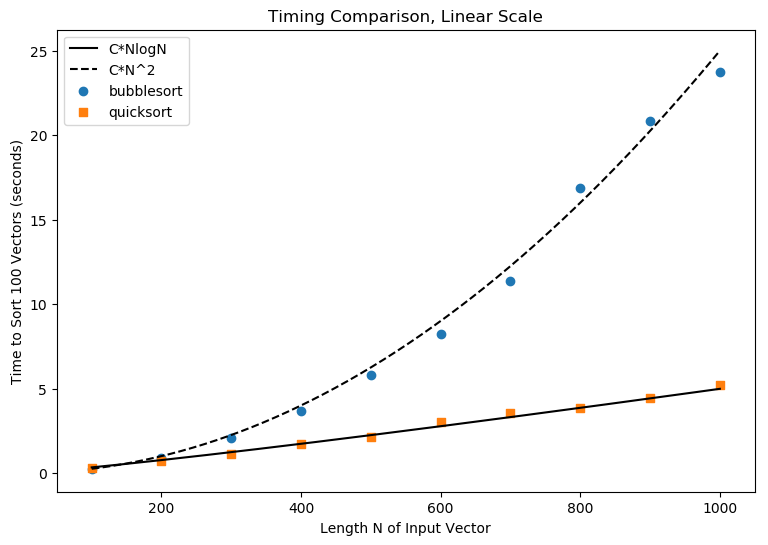
\includegraphics[width=0.6\textwidth]{hw1/fig3.png}
\end{figure}
The difference can be seen immediately between the two algorithms, but to highlight the difference in the actual curvature of the two trends, not just their relative scales, we can plot them with a log-scaled yaxis: \par
\begin{figure}[h]
\centering
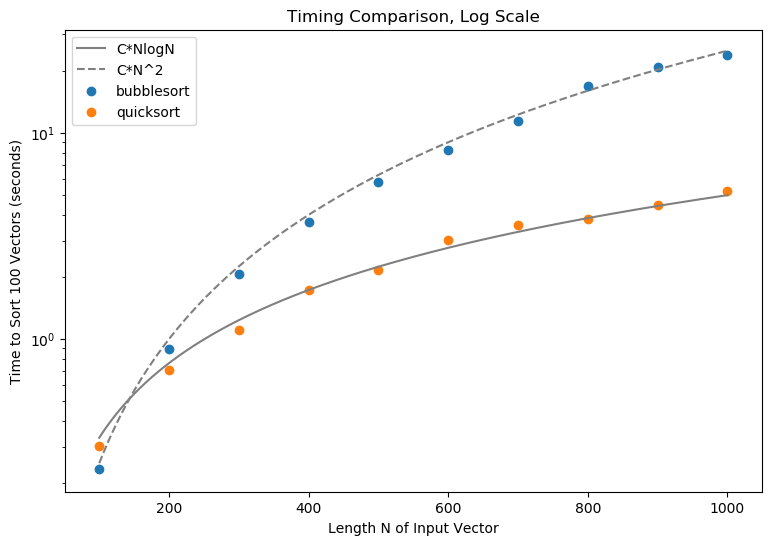
\includegraphics[width=0.6\textwidth]{hw1/fig4.png}
\end{figure}
For the assignments and conditionals, the same pattern is evident, and again, moving to a log-scaled y-axis makes the differences in curvature more apparent: \par
\begin{figure}[h!]
\centering
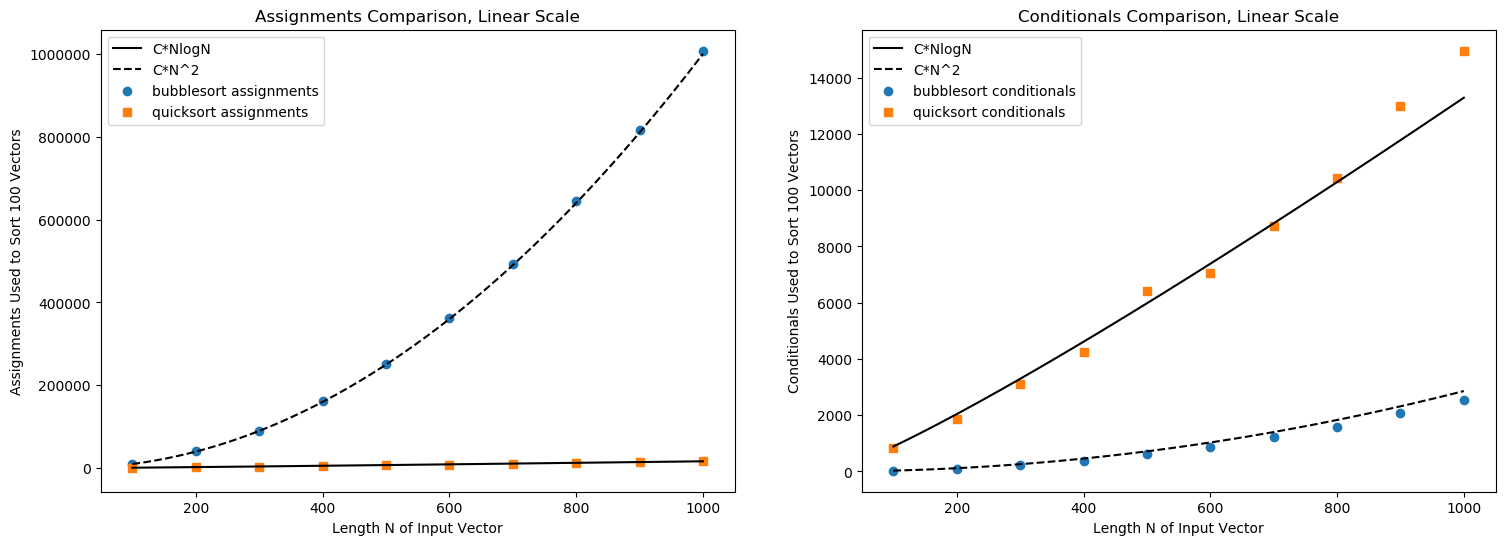
\includegraphics[width=\textwidth]{hw1/fig1.png}
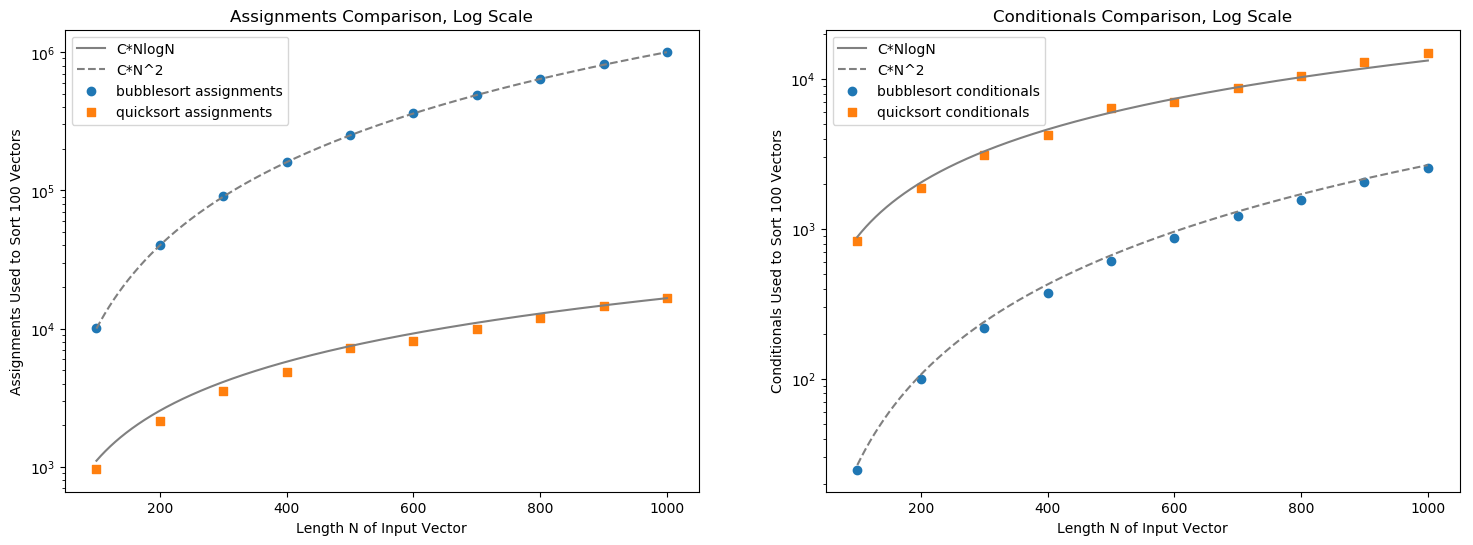
\includegraphics[width=\textwidth]{hw1/fig2.png}
\end{figure}
Unlike with the raw time or the assignments counts, We note that for the conditionals, QuickSort's counts are higher than that of BubbleSort. This is not counter to our original hypothesis, however, since the curvature is still more closely aligned with a logarithmic function than a quadratic; furthermore, the difference in raw values is easily manipulated with scalar multiplication: \par
\begin{figure}[h!]
\centering
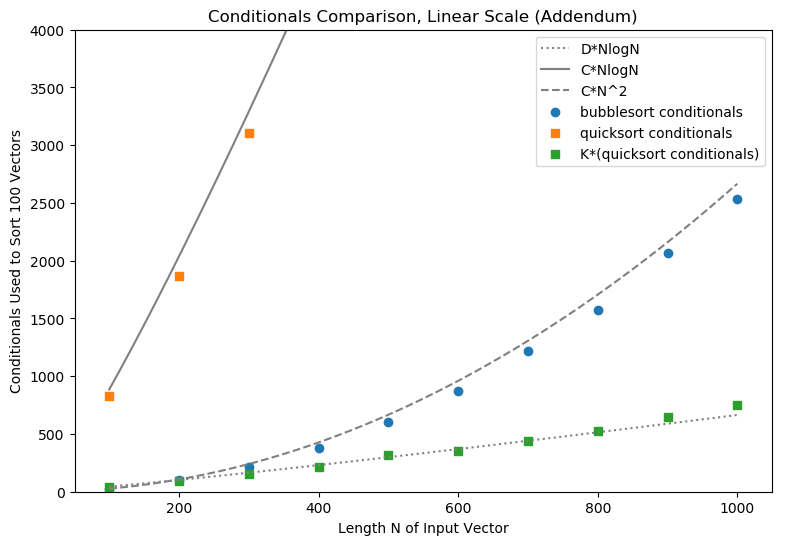
\includegraphics[width=0.6\textwidth]{hw1/fig5.png}
\end{figure}
Indeed, looking at the code in Section 1, we can see that while QuickSort costs more conditionals per iteration than BubbleSort, BubbleSort runs more iterations overall (on average), leading to the steeper curve in all three measures of complexity for BubbleSort relative to Quicksort. \par

\section{Github Repository}
All of the code used in this assignment is on Github: \url{https://github.com/laueste/algorithms-ucsf-2019}
\end{document}